\documentclass[bwprint]{gmcmthesis}
\usepackage{amsmath}
\numberwithin{figure}{section}
\renewcommand{\thefigure}{\arabic{section}-\arabic{figure}} 
% \documentclass[withoutpreface,bwprint]{cumcmthesis}
% 去掉封面与编号页

\title{中国研究生数学建模竞赛论文标题}
\baominghao{No.00000001} %参赛队号
\schoolname{XX大学/学院}%学校名称
\membera{队员A} %队员A
\memberb{队员B} %队员B
\memberc{队员C} %队员C
\begin{document}
 \maketitle
 \begin{abstract}
概述
\par 针对问题一
\par 针对问题二
\par 针对问题三
\par 最后,基于模型预测出的结果,我们总结出了一些有利于控制病毒传播的策略,并写成给上海政府的建议书。






\keywords{针对具体的问题列一到两个关键字\quad  建模算法列出\quad }
\end{abstract}

%\pagestyle{plain}

%目录
\tableofcontents

\section{问题背景与问题重述}
\subsection{问题背景}
2019年底爆发的新冠肺炎疫情给全人类带来深重苦难,至今已有4亿多人感染,6000多万人死亡。面对突如其来的疫情,中国政府始终将人民生命财产安全放在第一位,果断采取科学防控措施,有效遏制了疫情大面积蔓延,有力改变了病毒传播的危险进程,最大限度保护了人民生命安全和身体健康。直至2022年初,我国的新冠肺炎疫情已得到基本控制。
\par 然而,在2022年3月上海突然爆发了奥密克戎疫情,直到现在疫情仍未得到根本控制,使得疫情防控态势又紧张了起来。面对疫情,需要我们采取科学防控措施,利用已经公布的相关数据和数学模型,对本轮上海新冠肺炎疫情进行预测,使人们更好的认识新冠肺炎传播规律,也能为相关部门采取防控措施提供参考,对疫情防控具有积极作用。

\subsection{问题重述}
题目提示需要在分析上海市卫生健康委员会和国家卫生健康委员会通报的实时疫情数据的基础上(主要包括累计报告病例、累计治愈病例、累计死亡病例、跟踪隔离人数、单日新增确诊病例等),建立新冠肺炎传播模型以预测未来疫情发展趋势并评估防疫策略。
\begin{enumerate}
\item
问题1:搜集有关美国国内疫情应对措施,分析在此防控措施下造成的美国疫情蔓延态势。若上海采取相同防控措施,通过建立模型分析疫情蔓延情况及可能带来的严重后果。
\item 问题2:疫情爆发初期,上海市政府采取精准防控策略并公布了相关数据,需要分析上述数据以建立数学模型预测在该措施下的再生数。通过前面建立的模型预测两个月内疫情发展趋势和累计病例数。
\item 问题3:随着疫情发展趋势,上海市政府加强了管控措施,积极推行如:全员核算、启用方舱医院接收轻型患者和无症状感染者等措施。需要根据对应的公布数据,建立恰当的数学模型预测包括:流行时间、流行规模等指标在内的本次疫情发展趋势。预测完成后还需要根据五月份的数据来验证模型的有效性。若上海疫情在五月中旬之后仍未结束,需要根据模型预测一周内疫情发展趋势。
\item 问题4:根据建模结果,总结出一些对抗击疫情有积极作用的针对性建议,给有关部门进行参考。
\end{enumerate}



\section{模型假设}
\begin{enumerate}
\item 假设气候因素(温度、湿度)对病毒传播无影响
\item 假设人口总数在预测区间内恒定
\item 假设个体对病毒的易感性相同
\item 假设病毒传染性不变
\end{enumerate}





\section{符号说明}
\begin{tabular}{cc}
 \hline
 \makebox[0.4\textwidth][c]{符号}	&  \makebox[0.5\textwidth][c]{意义} \\ \hline
 	$N_a$	    & 宽度(cm) \\ \hline
	$S_a$	    & 宽度(cm) \\ \hline
	$E_a$	    & 宽度(cm) \\ \hline
	$I_{S,a}$	    & 宽度(cm) \\ \hline
	$I_{S,a}^{drug}$	    & 宽度(cm) \\ \hline
	$I_{S,a}^{naive}$	    & 宽度(cm) \\ \hline
	$I_{A,a}$	    & 宽度(cm) \\ \hline
	$H_a$	    & 宽度(cm) \\ \hline
	$H_{N,a}$	    & 宽度(cm) \\ \hline
	$ICU_a$	    & 宽度(cm) \\ \hline
    $\lambda_a$	    & 宽度(cm) \\ \hline
    $\beta$	    & 宽度(cm) \\ \hline
    $\phi$	    & 宽度(cm) \\ \hline
    $r_a$	    & 宽度(cm) \\ \hline
    $M$	    & 宽度(cm) \\ \hline
    $CM$	    & 接触矩阵 \\ \hline
    $\beta$	    & 宽度(cm) \\ \hline
    $\beta$	    & 宽度(cm) \\ \hline
 	L	           & 长度(cm)  \\ \hline
\end{tabular}

\section{问题分析}
\subsection{对上海疫情情况的调研}
为了给对模型的分析提供参考,需要首先对上海疫情近期的发展情况以及政策变动进行调研。经过对近期新闻的搜集和整理,绘制疫情曲线和政策变动图如下所示
\begin{figure}[!h]
\centering
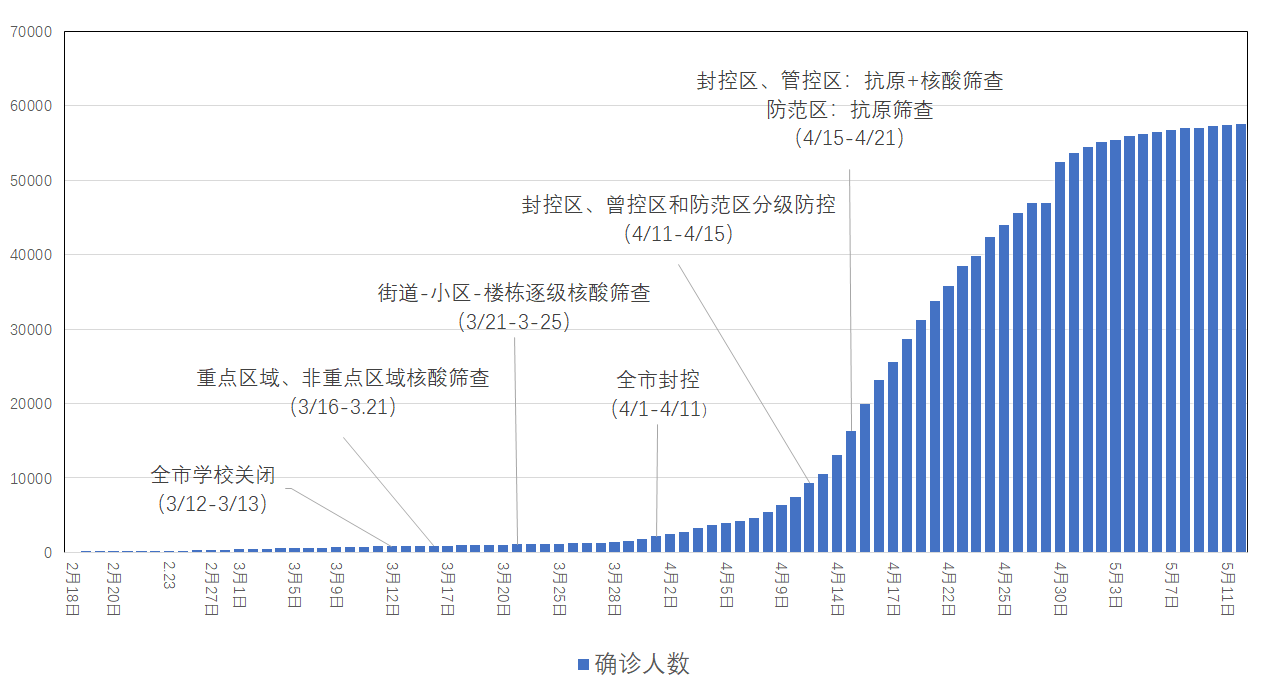
\includegraphics[width=.9\textwidth]{shanghai_bianhua.png}
\caption{上海防控政策的变化和疫情曲线}
\label{fig3}
\end{figure}
\par 本轮奥密克戎疫情爆发以来,上海市陆续升级公共卫生干预措施对疫情进行管控。3 月12 日起,全市中小学调整为线上教学,幼儿园、托儿所停止入园,大学封闭。从3 月16 日起,对社区逐级开展“街镇-小区-楼栋”的区域化、网格化核酸筛查;3 月28 日5 时起浦东、浦南及毗邻区域实施封控,开展核酸筛查;4 月1 日开始全市封控;4 月10 日后划分封控区、管控区和防范区进行分级防控,因地制宜采取不同的防疫检测和防控措施。
\subsection{对问题一的分析}
问题一要求预测出上海在采取美国式“躺平”防疫政策的情况下会出现的疫情情况。首先我们需要对美国的防控策略进行调查,并利用现有的美国疫情数据推算出模型参数。最后将确定了参数的模型应用在上海的场景下,从而预测出可能的疫情规模。流程图如下所示
\subsection{对问题二的分析}
问题二要求根据上海市政府初期的精准防控策略,估计本次疫情的发展规模,并且估计在此策略下的再生数。
\subsection{对问题三的分析}
问题三要求预测在上海实施了严格防疫管控措施的情况下的疫情趋势。
\section{数学模型}
介绍主流的方法
时间序列方法、机器学习方法、传统方法(SIR模型及其变种)
\subsection{相关概念}
\subsubsection{再生数 Reproduction Number}
再生数是
\par 基本再生数是
\par 实际再生数是
\subsubsection{感染率 Force of Infection}
感染率
\subsubsection{隔间模型 Compartment model}
常用的模型是隔间模型

\subsection{SIR模型}
SIR模型的基本表达式:
\begin{equation} \label{}
\begin{aligned}
        &\frac{dS\left( t \right)}{dt}=-\frac{\lambda S\left( t \right) I_p\left( t \right)}{N}\\
        &\frac{dI\left( t \right)}{dt}=\frac{\lambda S\left( t \right) I_p\left( t \right)}{N}-\mu I\left( t \right)\\
        &\frac{dR\left( t \right)}{dt}=\mu I\left( t \right)\\
\end{aligned}
\end{equation}

\par
其中一些基本符号的解释如下表所示:

\begin{tabular}{cc}
    \hline
    \makebox[0.4\textwidth][c]{符号}	&  \makebox[0.5\textwidth][c]{意义} \\ \hline
    $S_p\left( t \right) $    & $t$时刻预测的易感人数(人)  \\ \hline
    $I_p\left( t \right) $ 	& $t$时刻预测的感染人数(人)  \\ \hline
    $R_p\left( t \right) $ 	& $t$时刻预测的治愈人数(人)  \\ \hline
    $N$	                        & 总人数(人)  \\ \hline
    $\lambda$ 	                & 宽度(人) \\ \hline
    $\mu$	                    & 长度(人)  \\ \hline
\end{tabular}

其中:
\begin{equation} \label{}
    N\,\,=\,\,S_p\left( t \right) +I_p\left( t \right) +R_p\left( t \right) 
\end{equation}

\subsection{SLIRS模型}
SLIRS(Susceptible-Lantent-Infectious-Removed-Susceptible)模型是对SIR模型的拓展。相比于基础的SIR模型,SLIRS主要考虑到病毒携带者、因病去世者的存在以及康复者可能会反复感染。将人群分成了以下几种:
\begin{enumerate}
\item 易感人群(Susceptible)$S$指会被感染的人群
\item 病毒携带人群(Lantent/Exposed)$E$指与感染者接触,但尚未感染的人群。这一类人群没有传染性,但会在一定时间内变为感染者。
\item 感染者(Infectious)$I$指被病毒感染的人群,这类人一定具有传染性。根据症状有无,可以进一步分成无症状感染者(asymptomatic infectious)$I_a$和有症状感染者(symptomatic infectious)$I_s$。无症状感染者一般情况下不需要住院就能自愈,变为康复者;而有症状感染者根据病情严重性,在医疗资源足够的情况下,会进入普通病房或ICU病房
\item 康复者(Recovered)$R$指刚从感染状态恢复健康的人群。这一类人因为曾被感染因而对病毒有较高的免疫力,但随着时间发展,其免疫力会逐步下降,最终转变为易感人群。
\item 因病去世者(Deceased)$D$
\item 住院病人(Hospitalized)$H$,可进一步划分为普通病房(包含方舱医院)病人和ICU病房病人。基于合理假设,这一类人通常不再有传染性,但可能会因病离世。

\end{enumerate}
\par 本文模型考虑到了病毒在不同年龄段中的传播特性、致病率、致死率等特性的差异,按14个年龄段划分人群。在人群中展开疫苗接种,能产生一定免疫效果,降低致病率和致死率;与此同时,采用疫苗种类、接种剂数、疫苗免疫效果的时变特性会带来抗病毒效果的差异。因此,本模型同时将。。。考虑抗病毒药物的效果,。。。
\par 采用随机模型,符合二项分布。对每一个个体,其
\subsubsection{年龄段的划分}
将人群按年龄段划分
\subsubsection{接触矩阵}
接触矩阵表述了不同年龄人群之间的接触频次。接触矩阵每一点的值$CM_{ij}$表示年龄段$i$平均每天接触到年龄段$j$的人数。即

Dina等人的论文给出了对中国人口接触矩阵的估计
\par 当政府实行管控措施时,会直接影响到接触矩阵的值。比如,当实行学校关闭的政策时,青少年年龄段的接触矩阵值会大幅减小;当实行全方面封控的时候,整个接触矩阵的值都会减小。接触矩阵的变化反应了管控措施的变化。
\par 研究表明,相对于封锁期间,解封后平均每人每日接触人数恢复了5\%至17\%,但仍低于流行前接触水平的3-7倍。放松干预措施后大部分接触仍发生在家庭内部,工作场所和社区(家庭、学校、工作场所以外)的接触有所恢复,但家庭内部典型的同龄人接触和两代人接触的特征仍然在接触矩阵中占主导地位(图2)。
\subsubsection{医疗资源}
医疗资源的数量决定了社会对疫情的承受能力,当疫情处于高峰时期并且医疗资源不足时会出现医疗挤兑的情况,从而造成重症率和死亡率的提高。
\par 假定在医院中,病毒不会进一步传播
\begin{figure}[!h]
\centering
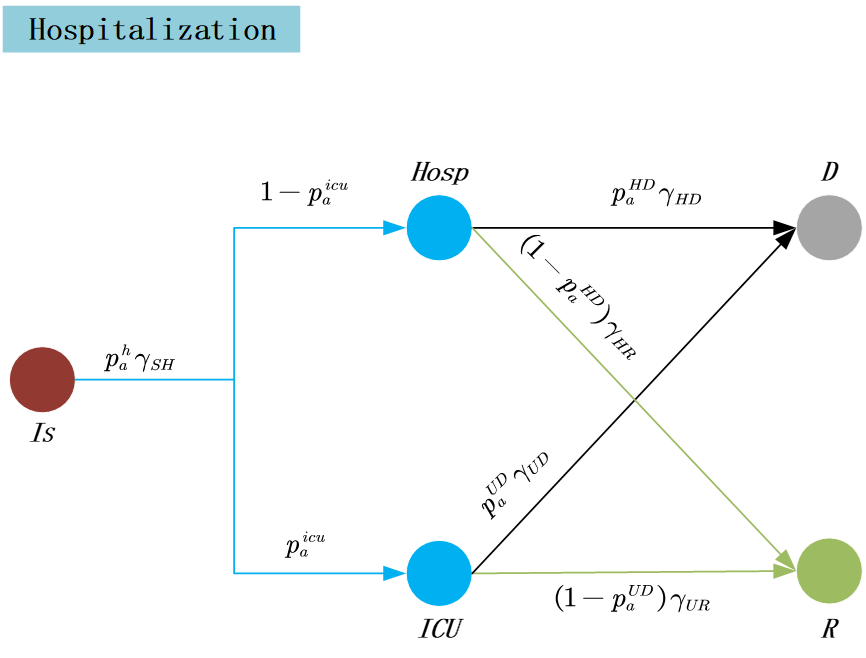
\includegraphics[width=.75\textwidth]{hospital.png}
\caption{上海防控政策的变化和疫情曲线}
\label{fig3}
\end{figure}
\subsubsection{药物治疗}
抗病毒药物的使用能减轻病情,降低住院率、死亡率,缩短康复时间。本模型考虑抗病毒药物的效果,将有症状感染者划分为两类:一类是定期使用抗病毒药物的;另外一类不使用抗病毒药物。使用抗病毒药物的患者比例为$p_a^{drug}$。
\subsubsection{疫苗}
考虑
\subsubsection{隔间模型状态转变的随机链式过程}
\begin{figure}[!h]
\centering
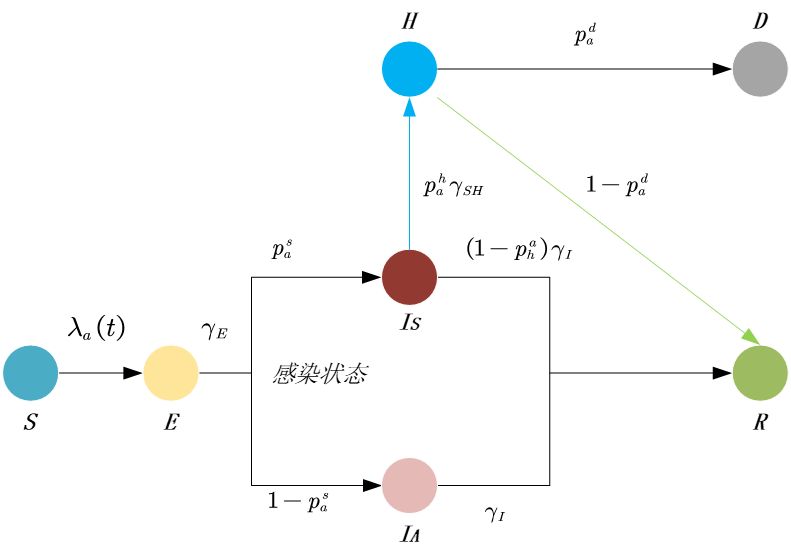
\includegraphics[width=.75\textwidth]{seirhd.png}
\caption{上海防控政策的变化和疫情曲线}
\label{fig3}
\end{figure}

\begin{figure}[!h]
\centering
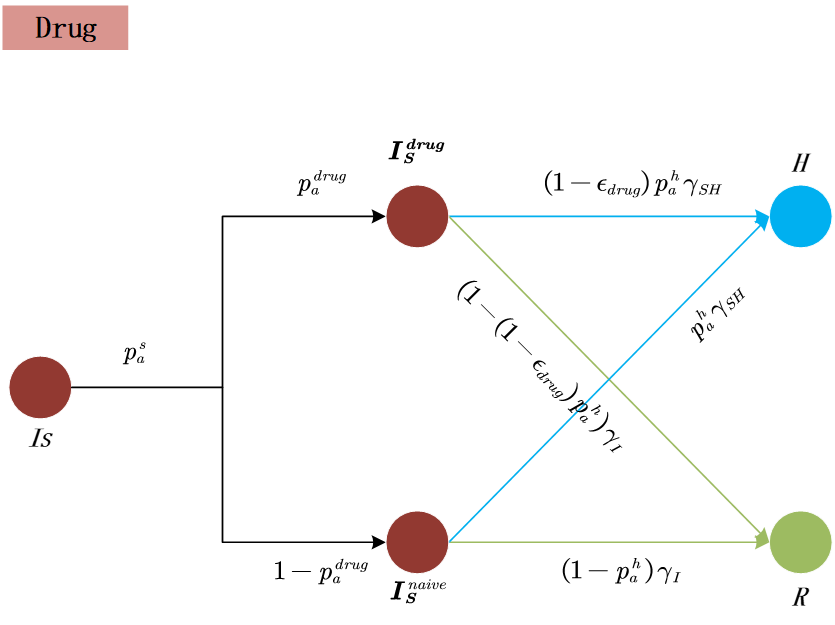
\includegraphics[width=.75\textwidth]{Drug.png}
\caption{上海防控政策的变化和疫情曲线}
\label{fig3}
\end{figure}



\begin{figure}[!h]
\centering
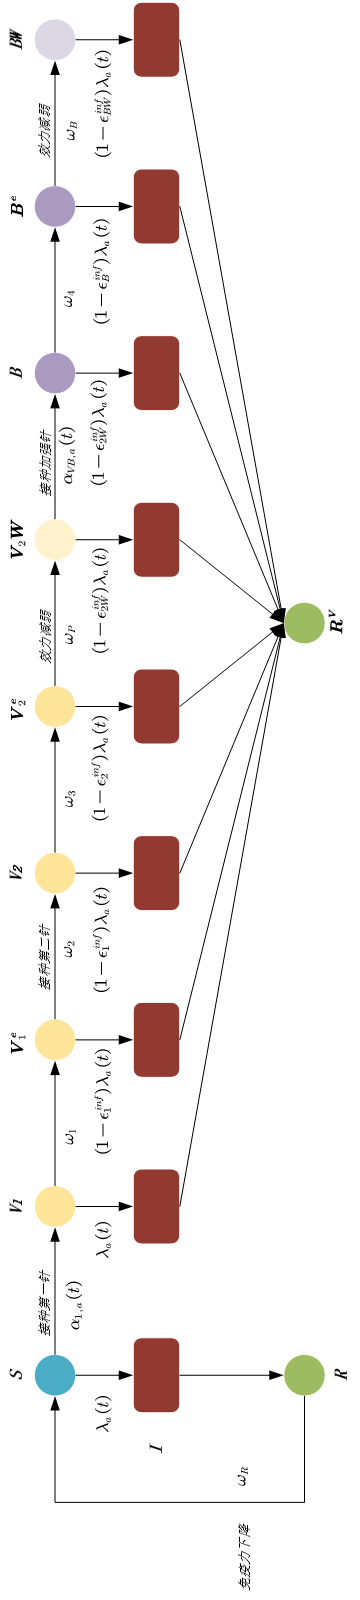
\includegraphics[width=0.36\textwidth]{vaccine.png}
\caption{上海防控政策的变化和疫情曲线}
\label{fig3}
\end{figure}

\par 状态的转变均符合二项分布
对于每一个易感者个体,其
\begin{equation}
\Delta S^e_a(t)\sim B(S_a(t),1-e^{-\lambda_a(t)})
\end{equation}
\begin{equation}
\lambda_a(t)=\frac{1}{T}\sum_jCM_{aj}\cdot\beta\frac{I}{N}
\end{equation}
\subsection{考虑大规模疫苗接种的模型}
\subsubsection{时间线分析}

对于美国的疫情数据
对于中国的疫情数据



问题二要求上海在实行初期“精准防控”策略下的疫情发展趋势,并且估算出再生数。
SEIR模型
机器学习方法,时间序列方法
缺乏可解释性

\section{问题求解}
\subsection{数据搜集与预处理}
数据来源为“Our World In Data”网站。
本文使用了BFGS算法来进行 $\lambda$ 与 $\mu$ 的计算。
根据我们现有的美国奥密克戎毒株的有关数据,可以根据这些数据求出相应的参数。那么,可以求解下面的最小二乘问题以估计曲线的参数:
\begin{equation} \label{}
    \underset{\lambda ,\mu}{\min}\frac{1}{2}\underset{t=1}{\overset{T}{\varSigma}}\left\| I_r\left( t \right) -I_p\left( t \right) \right\| ^2
\end{equation}
其中
\subsection{对问题一的求解}
\subsection{对问题二的求解}
\subsubsection{再生数的估计}
对于SIR模型,再生数可以直接求出
\subsection{对问题三的求解}

\section{建议信}
致中共上海市委、上海市人民政府的一封信

尊敬的中共上海市委、上海市人民政府:
我们是来自南京理工大学的三名研究生,有幸在南京理工大学研究生数学建模竞赛中遇到了上海市疫情预测模型相关的一道题目,通过查阅相关资料、进行数据调试,我们提出了基于XXXXXXXX的新冠肺炎预测模型,并对上海市前期的疫情数据有较好的拟合效果。所以我们将研究结果以书信形式传达,希望能够为上海市的疫情防控奉献我们的一份力量。
自从2022年3月1日上海市此轮本土疫情爆发开始,就获取了全国人民的广泛关注。上海作为一个拥有者2500万常住人口的超大城市。
根据我们的预测所构建的预测模型,将为上海市防疫政策提出以下建议:
一、给每一个被隔离的居民发放精神抚慰补贴。首先,上海绝大多数隔离点环境一般,有的临时搭好的,环境很差,不利于休息与康复。因为疫情发展太快,来不及在住宿问题上满足大家的基本要求,我们都理解,所以需要用补贴来安抚人心。同时也是为疫情控制不力,向那些被隔离者的补偿,这才是老百姓需要的实实在在的道歉,不能只放在嘴上。补贴可以分成三部分,一部分是固定的精神抚慰金,一视同仁,另一个是住宿补贴,可以把所有隔离点分成若干档次,入住高档次的补贴少一点,住得差的补多一点,公平公正。第三个是密接观察补贴,有很多人没有得病,但因为是密接者,也被拉走隔离观察,很有可能原本没事,但隔离点人员复杂,最后阴变阳,所以这些人可以得到第三部分的补贴。这里要申明一下,配合防疫是市民的义务,既然市民为了防疫做出牺牲,得到一定的补偿合情合理。
二、由于政府免费发放的物资有限,靠这些东西远远不够,所以团购抢菜成了所有上海市民每天必做的事情。但现在任何一个团购套餐价格偏贵,几乎都要翻倍,这是事实,而且很难管,你管控价格,别人不卖了,你能如何?我建议相关部门给每户居民“额外成本支出”的补贴,以三口之家平均一个月生活支出为基数,提供50\%的补贴。比如三口之家一个月要花2000元的口粮,以目前物价涨幅来算的话,要多花1000元,这部分由政策买单。
三、在每个小区招募“有偿服务人员”。现在很多小区都是志愿者在给大家送东西。所有物资放在小区门口消杀,然后由志愿者送到各栋大楼,工作量太大了。很多小区的业主会主动给志愿者小费,但管理很乱,不统一。建议每个小区安排一定数量的“有偿服务人员”,每天给予补贴,由政策统一买单,这样皆大欢喜,有人干活。
四、严管各居委会、业委会中饱私囊的行为。很多人利用自己的职权,筛选进入小区团购的供应商,给好处的,便给予方便,没有好处的拒之门外,或层层设防。这些我们也理解,毕竟现在基层最苦,什么事都落在居委会头上,他们从中获利很正常,只是这样的行为让居民无法公正的获取合理的食物,利己可以,但不能损人。建议给每个居委会一些临时津贴,高薪养廉。让所有合规的团购物资进入小区,一视同仁。这样也可以变相控价。否则一家独大,价格随便开。
五、开放更多物资提供点,释放几万外卖员的运输力,让网购不需要抢。
以上五个方面如果不能妥善处理,容易引发民众不安情绪,不利于各小区内部稳定。上海已经在疫情初期走了弯路,要吸取教训,而这些举措可以避免次生灾害,让市民安安心心完成抗疫重任。
对未来的展望:
上海疫情失控后防疫压力大、难度高,我们都理解。现在不是指责的时候,是正面解决问题的关键时刻。
3月22日国家卫健委新冠肺炎疫情应对处置工作领导小组专家组组长梁万年表示,社区在执行防疫政策的过程中,要特别强调“有温度”。
    我们曾去过许多次上海,去看过绚丽的霓虹灯下东方明珠的辉煌、黄浦江上耀眼的光芒却有一种近代的沧桑、弄堂中老上海人将油灯点亮,星星点点照亮长廊,临街的商铺里是闪亮的衣裳,美丽的上海让我们如此沉醉,虽许久不见,但仍想念那人流如潮、车水马龙的繁华与奔忙。

愿:
上海一切安好,所有上海人民早日走出疫情阴霾


几名持续关注上海疫情的南理工学子
白宇铖 李文睿 马寅锐
2022年 5月 16日


\section{模型的评价}
\subsection{模型的优点}
模型的优点模型的优点模型的优点模型的优点模型的优点模型的优点模型的优点模型的优点模型的优点模型的优点模型的优点模型的优点模型的优点模型的优点。
\subsection{模型的缺点}
模型的缺点模型的缺点模型的缺点模型的缺点模型的缺点模型的缺点模型的缺点模型的缺点模型的缺点模型的缺点模型的缺点模型的缺点模型的缺点模型的缺点。



\section{写作参考格式}
写作过程中可能要用到一些格式参考,正式写作的时候,可以直接将这一章删掉即可。

\textbf{无序列表格式}
\begin{itemize}
\item 无序列表1
\item 无序列表2
\item 无序列表3
\item 无序列表4
\end{itemize}


\textbf{表格格式}

\begin{tabular}{cc}
 \hline
 \makebox[0.4\textwidth][c]{符号}	&  \makebox[0.5\textwidth][c]{意义} \\ \hline
 D	    & 宽度(cm) \\ \hline
 L	    & 长度(cm)  \\ \hline
\end{tabular}


%
%\textbf{图片格式}
%\begin{figure}[h]
%\centering
%\includegraphics[width=5cm]{xxx.jpg}
%\caption{图片标题}
%\end{figure}

\section{参考文献}
%参考文献
\begin{thebibliography}{1.2}%宽度9
\setlength{\itemsep}{-2mm}
 \bibitem{bib:one} 
 韩中庚. 数学建模方法及其应用[M]. 高等教育出版社, 2005.
 \bibitem{bib:two}
 韩中庚. 数学建模方法及其应用[M]. 高等教育出版社, 2005.
  \bibitem{bib:two}
 韩中庚. 数学建模方法及其应用[M]. 高等教育出版社, 2005.
\end{thebibliography}

\newpage
%附录
\appendix
\section{程序代码}
%设置不同语言即可。
\begin{lstlisting}[language=Matlab] 
kk=2;[mdd,ndd]=size(dd);
while ~isempty(V)
[tmpd,j]=min(W(i,V));tmpj=V(j);
for k=2:ndd
[tmp1,jj]=min(dd(1,k)+W(dd(2,k),V));
tmp2=V(jj);tt(k-1,:)=[tmp1,tmp2,jj];
end
tmp=[tmpd,tmpj,j;tt];[tmp3,tmp4]=min(tmp(:,1));
if tmp3==tmpd, ss(1:2,kk)=[i;tmp(tmp4,2)];
else,tmp5=find(ss(:,tmp4)~=0);tmp6=length(tmp5);
if dd(2,tmp4)==ss(tmp6,tmp4)
ss(1:tmp6+1,kk)=[ss(tmp5,tmp4);tmp(tmp4,2)];
else, ss(1:3,kk)=[i;dd(2,tmp4);tmp(tmp4,2)];
end;end
dd=[dd,[tmp3;tmp(tmp4,2)]];V(tmp(tmp4,3))=[];
[mdd,ndd]=size(dd);kk=kk+1;
end; S=ss; D=dd(1,:);
 \end{lstlisting}


\end{document} 